\documentclass[12pt]{article}
\usepackage[utf8]{inputenc}
\usepackage{graphicx} % Allows you to insert figures
\usepackage{subcaption}
\usepackage{amsmath} % Allows you to do equations
\usepackage{fancyhdr} % Formats the header
\usepackage{geometry} % Formats the paper size, orientation, and margins
\usepackage{dirtytalk} % typesetting different types of quotation
\usepackage[english]{babel}
\usepackage{csquotes}
\usepackage{hyperref}
\usepackage{listings}
\usepackage{xcolor}
\usepackage{array}
\usepackage{caption}

% Define code style
\lstset{
  basicstyle=\ttfamily\small,
  backgroundcolor=\color{gray!10},
  frame=single,
  breaklines=true,
  postbreak=\mbox{\textcolor{red}{$\hookrightarrow$}\space},
  keywordstyle=\color{blue},
  commentstyle=\color{green!50!black},
  stringstyle=\color{orange},
}


\linespread{1.25} % About 1.5 spacing in Word
\setlength{\parindent}{0.8cm} % No paragraph indents
\setlength{\parskip}{0em} % Paragraphs separated by one line
\renewcommand{\headrulewidth}{0pt} % Removes line in header
\geometry{a4paper, portrait, margin=1in}
\setlength{\headheight}{14.49998pt}
\graphicspath{ {images/} }

\begin{document}
\begin{titlepage}
   \begin{center}
    \textsc{\large Ministry of Education of Republic of Moldova}\\[0.5cm]
    \textsc{\large Technical University of Moldova}\\[0.5cm]
    \textsc{\large Faculty of Computers, Informatics and Microelectronics}\\[0.5cm]
    \textsc{\large Department of Physics}\\[1.2cm]
    
    \vspace{25 mm}
    
    \textsc{\Large Criptography and security}\\[0.5cm]
    \textsc{\large Laboratory work \#2}\\[0.5cm]    % <<<<<<< CHANGE LAB NUMBER HERE
    
    \newcommand{\HRule}{\rule{\linewidth}{0.5mm}}
    \vspace{10 mm}
    \HRule \\[0.4cm]
    { \LARGE \bfseries Cryptanalysis of monoalphabetic ciphers.}\\[0.4cm] % <<<<<<< CHANGE LAB TITLE HERE
    \HRule \\[1.5cm]
    
    \vspace{10mm}
    
    \begin{minipage}[t]{0.4\textwidth}
    \begin{flushleft} \large
    \emph{Author:} \\
    Dmitrii \textsc{Belih}\\                         % <<<<<<< CHANGE YOUR NAME HERE
    std. gr. FAF-232                                % <<<<<<< CHANGE GROUP NUMBER HERE
    \end{flushleft}
    \end{minipage}
    ~
    \begin{minipage}[t]{0.4\textwidth}
    \begin{flushright} \large
    \emph{Verified:} \\
    \textsc{Zaica} M.\\
    \end{flushright}
    \end{minipage}\\[3cm]
    
    \vspace{5 mm}
    \large Chișinău 2025\\[0.5cm]
    
    \vfill
    \end{center}
\end{titlepage}

\setcounter{page}{2}
\pagestyle{fancy}
\fancyhf{}
\rhead{\thepage}
\lhead{FAF-232 Belih Dmitrii; Laboratory Work №2}




% \section*{Introduction}
\section*{Theory Background}
\hspace{0.8cm}

The weak point of monoalphabetic encryption systems lies in the frequency of appearance of characters in the text. If an encrypted text is long enough and the language in which the plaintext is written is known, the system can be broken by an attack based on the frequency of appearance of letters in a language (frequency analysis attack), this frequency being an intensively studied problem (not necessarily for cryptographic purposes) and as a result various ordering structures have been built relative to the frequency of appearance of letters in each European language and in other languages. Usually, the longer an encrypted text is, the closer the frequency of the letters used is to this general ordering. A comparison between the two ordering relationships (that of the characters in the encrypted text and that of the letters in the current language alphabet) leads to the realization of several correspondences (plaintext letter – ciphertext letter), which uniquely establishes the encryption key.
\begin{table}[h!]
    \centering
    \caption{Frecvența literelor limbii engleze}
    \label{tab:freq_eng}
    \begin{tabular}{|c|c|c|c|c|c|c|c|c|c|c|c|c|}
        \hline
        \textbf{A} & \textbf{B} & \textbf{C} & \textbf{D} & \textbf{E} & \textbf{F} & \textbf{G} & \textbf{H} & \textbf{I} & \textbf{J} & \textbf{K} & \textbf{L} & \textbf{M} \\
        \hline
        8.17 & 1.49 & 2.78 & 4.25 & 12.7 & 2.23 & 2.01 & 6.09 & 6.97 & 0.15 & 0.77 & 4.03 & 2.41 \\
        \hline
        \textbf{N} & \textbf{O} & \textbf{P} & \textbf{Q} & \textbf{R} & \textbf{S} & \textbf{T} & \textbf{U} & \textbf{V} & \textbf{W} & \textbf{X} & \textbf{Y} & \textbf{Z} \\
        \hline
        6.75 & 7.51 & 1.93 & 0.095 & 5.99 & 6.33 & 9.06 & 2.76 & 0.98 & 2.36 & 0.15 & 1.97 & 0.07 \\
        \hline
    \end{tabular}
    \parbox{\textwidth}{\small \textit{Pentru limba engleză avem situația prezentată în tabelul 2.2 și figura 2.2:}}
    \parbox{\textwidth}{\small \textit{Tabelul 2.2. Frecvența literelor limbii engleze}}
\end{table}
\begin{figure}[h!]
    \centering
    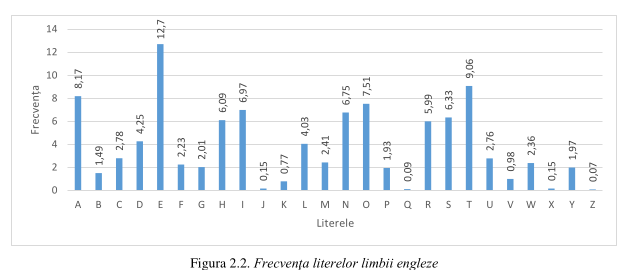
\includegraphics[width=0.8\textwidth]{img/Lom.png}
    \caption{Frequency of english letters}
    \label{fig:result1}
\end{figure}

\subsection*{Frequency analysis attack methodology}

We can use information about the frequency of letter occurrences in a language to attempt to break a monoalphabetic substitution cipher. This is possible because, for example, in a message written in English, the letter "E," which has the highest frequency, might be encrypted as "X." In that case, every "X" in the encrypted text would correspond to an "E" in the plaintext. Consequently, the most frequent letter in the encrypted text should be "X."

Thus, if we intercept an encrypted message and the most frequent letter in it is "P," we can assume that "P" was used to encrypt "E," and we can replace all "P"s with "E"s. Of course, not every text has exactly the same frequency, and as noted above, "T" and "A" also have high frequencies, so "P" could represent one of these. However, it is unlikely to be "Z," which is rarely encountered in English. By repeating this process with the next most frequent letter, we can make progress in breaking the message.

If we were to put all the letters in order and replace them according to the frequency table, it is most likely that we would not obtain the expected result. The cryptanalyst must use other "personality traits" of the letters to break the cryptogram. This may include examining pairs of letters (digraphs), the most common of which are TH, HE, AN, IN, ER, ON, RE, ED, ND, HA, AT, and EN. Triplets of letters (trigraphs) can also be very useful, with the most frequent in English being THE, AND, THA, ENT, ION, TIO, FOR, NDE, HAS, NCE, TIS, OFT, and MEN. Additionally, in English, only a few letters appear as doubles (SS, EE, TT, OO, and FF being the most frequent). There are only two meaningful single-letter words in English: "A" and "I."

Other frequent words also begin to emerge as we make some substitutions. For example, "T*E" may appear frequently after performing substitutions for "T" and "E." In this case, "T*E" is very likely to be "THE," a very common word in English.

The process of frequency analysis utilizes various subtle properties of the language, and for this reason, it is almost impossible for a computer to do all the work. Inevitably, a human element is necessary in this process to make informed decisions about which letters should be replaced.


\section*{The Task}

Either an encrypted message has been intercepted that is known to have been obtained using a monoalphabetic cipher. Applying the frequency analysis attack to find out the original message, assuming that it is a text written in English. Keep in mind that only the letters have been encrypted, the other characters remaining unencrypted.
\url{https://crypto.interactive-maths.com/frequency-analysis-breaking-the-code.html}

\textbf{My Variant: V2} \\
\textit{Wqv tooxwxng nc pvhivhf wn wqv witgpcniztwxngp uinodhvohifuwnjituqf. Widv, xw rtp zniv nc t
jtzv wqtg tgfwqxgj vspv—xw pndjqwwn ovstf hnzuivqvgpxng cni ngsf wqv pqniwvpw unppxasv
wxzv, gnw wqvsngjvpw—tgo wqv hifuwtgtsfpxp rtp, sxlvrxpv, edpw t udmmsv. Vjfuw'p rtpwqdp t
bdtpx hifuwnsnjf xg hngwitpw wn wqv ovtosf pvixndp phxvghv nc wnotf.Fvw jivtw wqxgjp qtkv
pztss avjxggxgjp, tgo wqvpv qxvinjsfuqp oxoxghsdov, wqndjq xg tg xzuvicvhw ctpqxng, wqv wrn
vsvzvgwp nc pvhivhf tgowitgpcniztwxng wqtw hnzuixpv wqv vppvgwxts twwixadwvp nc wqv
phxvghv. Tgopn hifuwnsnjf rtp anig. Xg xwp cxipw 3,000 fvtip, xw oxo gnw jinr pwvtoxsf.
Hifuwnsnjf tinpvxgovuvgovgwsf xg ztgf usthvp, tgo xg znpw nc wqvz xw oxvo wqv ovtwqp ncxwp
hxkxsxmtwxngp. Xg nwqvi usthvp, xw pdikxkvo, vzavoovo xg t sxwvitwdiv,tgo cinz wqxp wqvgvyw jvgvitwxng hndso hsxza wn qxjqvi svkvsp.Adw uinjivpp rtp psnr tgo evilf. Zniv rtp snpw wqtg
ivwtxgvo. Zdhq nc wqvqxpwnif nc hifuwnsnjf nc wqxp wxzv xp t utwhqrnil, t hitmf bdxsw
ncdgivstwvo xwvzp, puindwxgj, csndixpqxgj, rxwqvixgj. Ngsf wnrtio wqvRvpwvig Ivgtxpptghv
onvp wqv thhivwxgj lgnrsvojv avjxg wn adxso du tznzvgwdz. Wqv pwnif nc hifuwnsnjf odixgj
wqvpv fvtip xp, xg nwqvi rniop,vythwsf wqv pwnif nc ztglxgo. Hqxgt, wqv ngsf qxjq hxkxsxmtwxng
nc tgwxbdxwf wn dpv xovnjituqxhrixwxgj, pvvzp gvkvi wn qtkv ovkvsnuvo zdhq ivts hifuwnjituqf
—uviqtup cni wqtw ivtpng. Xg ngv htpv lgnrg cni zxsxwtif udiunpvp, wqv11wq-hvgwdif
hnzuxstwxng, Rd-hqxgj wpdgj-ftn ("Vppvgwxtsp cinz ZxsxwtifHstppxhp"), ivhnzzvgovo t widv xc
pztss hnov. Wn t sxpw nc 40 ustxgwvywxwvzp, itgjxgj cinz ivbdvpwp cni anrp tgo tiinrp wn wqv
ivuniw nc tkxhwnif, wqv hniivpungovgwp rndso tppxjg wqv cxipw 40 xovnjitzp nc tunvz. Wqvg,
rqvg t sxvdwvgtgw rxpqvo, cni vytzusv, wn ivbdvpw znivtiinrp, qv rtp wn Rixwv wqv hniivpungoxgj
xovnjitz tw t puvhxcxvo usthvng tg nioxgtif oxputwhq tgo pwtzu qxp pvts ng xw.Xg Hqxgt'p jivtw
gvxjqani wn wqv rvpw, Xgoxt, rqnpv hxkxsxmtwxngsxlvrxpv ovkvsnuvo vtisf tgo wn qxjq vpwtwv,
pvkvits cnizp nc pvhivwhnzzdgxhtwxngp rviv lgnrg tgo, t Uutivgwsf, uithwxhvo. Wqv Tiwqt-ptpwit,
t hstppxh rnil ng pwtwvhitcw twwixadwvo wn Ltdwxsft, xg ovphixaxgjwqv vpuxngtjv pvikxhv nc
Xgoxt tp uithwxhtssf ixoosxgj wqv hndgwif rxwqp Uxvp, ivhnzzvgovo wqtw wqv nccxhvip nc wqv
xgpwxwdwvp nc £ puxngtjv jxkvwqvxi puxvp wqvxi tppxjgzvgwp af pvhivw rixwxgj.Uviqtup znpw
xgwvivpwxgj wn hifuwnsnjxpwp, tztwvdi niuincvppxngts, xp wqtw Ktwpftftgt'p ctzndp wvywannl
nc vinwxhp, wqv Ltztpdwit,sxpwp pvhivw rixwxgj tp ngv nc wqv 64 tiwp, ni fnjtp, wqtw rnzvgpqndso
lgnr tgo uithwxhv. Wqv cndiwq jivtw hxkxsxmtwxng nc tgwxbdxwf, wqvZvpnun-wtzxtg, itwqvi
utitssvsvo Vjfuw vtisf xg xwp hifuwnjituqxhvknsdwxng, adw wqvg pdiutppvo xw. Wqdp, xg wqv
stpw uvixno nc hdgvxcnizrixwxgj, xg hnsnuqngp rixwwvg tw Didl (xg uivpvgw-otf Xitb) dgovi
wqvPvsvdhxo lxgjp xg wqv stpw cvr phniv fvtip avcniv wqv Hqixpwxtg vit,nhhtpxngts phixavp
hngkviwvo wqvxi gtzvp xgwn gdzavip. Wqvvghxuqvizvgw—xc pdhq xw av—ztf qtkv avvg ngsf cni
tzdpvzvgw ni wnpqnr ncc.}

\section*{Technical implementation}
\hspace{0.8cm}
First of all I need to analyze the frequency of letters in endlish text in my Variant. After using the provided tools I abserved this following photo
\begin{figure}[h!]
    \centering
    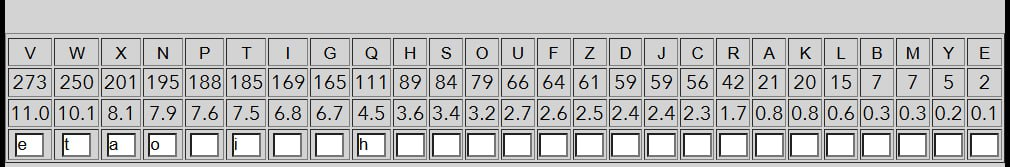
\includegraphics[width=0.8\textwidth]{img/Freq2.jpg}
    \label{fig:result1}
\end{figure}

Next step I can make comporision with the default frequency of english letter that wvreyone nows it. 

\begin{figure}[h!]
    \centering
    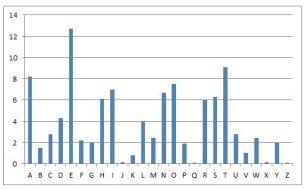
\includegraphics[width=0.8\textwidth]{img/def.png}
    \label{fig:result1}
\end{figure}

Now that we have all the letter frequencies in the ciphertext, we can start making some
substitutions. We see that the most frequent letter in the ciphertext is “V”, closely followed by “W”.
From the figure above, we can guess that these two letters represent “e” and
“t”, respectively, and after making these substitutions we get:
\\
\textit{tQe TOOXtXNG NC PeHIeHF tN tQe tITGPCNIZTtXNGP UINODHeOHIFUtNJITUQF. tIDe, Xt RTP ZNIe NC T JTZe tQTG TGFtQXGJ eSPe—Xt PNDJQttN OeSTF HNZUIeQeGPXNG CNI NGSF tQe PQNItePt UNPPXASe tXZe, GNt tQeSNGJePt—TGO tQe HIFUtTGTSFPXP RTP, SXLeRXPe, EDPt T UDMMSe. eJFUt'P RTPtQDP T BDTPX HIFUtNSNJF XG HNGtITPt tN tQe OeTOSF PeIXNDP PHXeGHe NC tNOTF.Fet JIeTt tQXGJP QTKe PZTSS AeJXGGXGJP, TGO tQePe QXeINJSFUQP OXOXGHSDOe, tQNDJQ XG TG XZUeICeHt CTPQXNG, tQe tRN eSeZeGtP NC PeHIeHF TGOtITGPCNIZTtXNG tQTt HNZUIXPe tQe ePPeGtXTS TttIXADteP NC tQe PHXeGHe. TGOPN HIFUtNSNJF RTP ANIG. XG XtP CXIPt 3,000 FeTIP, Xt OXO GNt JINR PteTOXSF. HIFUtNSNJF TINPeXGOeUeGOeGtSF XG ZTGF USTHeP, TGO XG ZNPt NC tQeZ Xt OXeO tQe OeTtQP NCXtP HXKXSXMTtXNGP. XG NtQeI USTHeP, Xt PDIKXKeO, eZAeOOeO XG T SXteITtDIe,TGO CINZ tQXP tQe GeYt JeGeITtXNG HNDSO HSXZA tN QXJQeI SeKeSP.ADt UINJIePP RTP PSNR TGO EeILF. ZNIe RTP SNPt tQTG IetTXGeO. ZDHQ NC tQeQXPtNIF NC HIFUtNSNJF NC tQXP tXZe XP T UTtHQRNIL, T HITMF BDXSt NCDGIeSTteO XteZP, PUINDtXGJ, CSNDIXPQXGJ, RXtQeIXGJ. NGSF tNRTIO tQeRePteIG IeGTXPPTGHe ONeP tQe THHIetXGJ LGNRSeOJe AeJXG tN ADXSO DU TZNZeGtDZ. tQe PtNIF NC HIFUtNSNJF ODIXGJ tQePe FeTIP XP, XG NtQeI RNIOP,eYTHtSF tQe PtNIF NC ZTGLXGO. HQXGT, tQe NGSF QXJQ HXKXSXMTtXNG NC TGtXBDXtF tN DPe XOeNJITUQXHRIXtXGJ, PeeZP GeKeI tN QTKe OeKeSNUeO ZDHQ IeTS HIFUtNJITUQF —UeIQTUP CNI tQTt IeTPNG. XG NGe HTPe LGNRG CNI ZXSXtTIF UDIUNPeP, tQe11tQ-HeGtDIF HNZUXSTtXNG, RD-HQXGJ tPDGJ-FTN ("ePPeGtXTSP CINZ ZXSXtTIFHSTPPXHP"), IeHNZZeGOeO T tIDe XC PZTSS HNOe. tN T SXPt NC 40 USTXGteYtXteZP, ITGJXGJ CINZ IeBDePtP CNI ANRP TGO TIINRP tN tQe IeUNIt NC TKXHtNIF, tQe HNIIePUNGOeGtP RNDSO TPPXJG tQe CXIPt 40 XOeNJITZP NC TUNeZ. tQeG, RQeG T SXeDteGTGt RXPQeO, CNI eYTZUSe, tN IeBDePt ZNIeTIINRP, Qe RTP tN RIXte tQe HNIIePUNGOXGJ XOeNJITZ Tt T PUeHXCXeO USTHeNG TG NIOXGTIF OXPUTtHQ TGO PtTZU QXP PeTS NG Xt.XG HQXGT'P JIeTt GeXJQANI tN tQe RePt, XGOXT, RQNPe HXKXSXMTtXNGSXLeRXPe OeKeSNUeO eTISF TGO tN QXJQ ePtTte, PeKeITS CNIZP NC PeHIetHNZZDGXHTtXNGP ReIe LGNRG TGO, T UUTIeGtSF, UITHtXHeO. tQe TItQT-PTPtIT, T HSTPPXH RNIL NG PtTteHITCt TttIXADteO tN LTDtXSFT, XG OePHIXAXGJtQe ePUXNGTJe PeIKXHe NC XGOXT TP UITHtXHTSSF IXOOSXGJ tQe HNDGtIF RXtQP UXeP, IeHNZZeGOeO tQTt tQe NCCXHeIP NC tQe XGPtXtDteP NC £ PUXNGTJe JXKetQeXI PUXeP tQeXI TPPXJGZeGtP AF PeHIet RIXtXGJ.UeIQTUP ZNPt XGteIePtXGJ tN HIFUtNSNJXPtP, TZTteDI NIUINCePPXNGTS, XP tQTt KTtPFTFTGT'P CTZNDP teYtANNL NC eINtXHP, tQe LTZTPDtIT,SXPtP PeHIet RIXtXGJ TP NGe NC tQe 64 TItP, NI FNJTP, tQTt RNZeGPQNDSO LGNR TGO UITHtXHe. tQe CNDItQ JIeTt HXKXSXMTtXNG NC TGtXBDXtF, tQeZePNUN-tTZXTG, ITtQeI UTITSSeSeO eJFUt eTISF XG XtP HIFUtNJITUQXHeKNSDtXNG, ADt tQeG PDIUTPPeO Xt. tQDP, XG tQe STPt UeIXNO NC HDGeXCNIZRIXtXGJ, XG HNSNUQNGP RIXtteG Tt DIDL (XG UIePeGt-OTF XITB) DGOeI tQePeSeDHXO LXGJP XG tQe STPt CeR PHNIe FeTIP AeCNIe tQe HQIXPtXTG eIT,NHHTPXNGTS PHIXAeP HNGKeIteO tQeXI GTZeP XGtN GDZAeIP. tQeeGHXUQeIZeGt—XC PDHQ Xt Ae—ZTF QTKe AeeG NGSF CNI TZDPeZeGt NI tNPQNR NCC
} \\

Next step is define the comon words so whe famous word is THE and we can see that where is the similar words like this. 
We now notice that the word "tQe" appears frequently in the passage. In English, the most common how I say 3-letter word is "the" and this fits with what we have already done, which suggests that the "Q" should be deciphered to "h".

And we have following text now:\\
\textit{the TOOXtXNG NC PeHIeHF tN the tITGPCNIZTtXNGP UINODHeOHIFUtNJITUhF. tIDe, Xt RTP ZNIe NC T JTZe thTG TGFthXGJ eSPe—Xt PNDJhttN OeSTF HNZUIeheGPXNG CNI NGSF the PhNItePt UNPPXASe tXZe, GNt theSNGJePt—TGO the HIFUtTGTSFPXP RTP, SXLeRXPe, EDPt T UDMMSe. eJFUt'P RTPthDP T BDTPX HIFUtNSNJF XG HNGtITPt tN the OeTOSF PeIXNDP PHXeGHe NC tNOTF.Fet JIeTt thXGJP hTKe PZTSS AeJXGGXGJP, TGO thePe hXeINJSFUhP OXOXGHSDOe, thNDJh XG TG XZUeICeHt CTPhXNG, the tRN eSeZeGtP NC PeHIeHF TGOtITGPCNIZTtXNG thTt HNZUIXPe the ePPeGtXTS TttIXADteP NC the PHXeGHe. TGOPN HIFUtNSNJF RTP ANIG. XG XtP CXIPt 3,000 FeTIP, Xt OXO GNt JINR PteTOXSF. HIFUtNSNJF TINPeXGOeUeGOeGtSF XG ZTGF USTHeP, TGO XG ZNPt NC theZ Xt OXeO the OeTthP NCXtP HXKXSXMTtXNGP. XG NtheI USTHeP, Xt PDIKXKeO, eZAeOOeO XG T SXteITtDIe,TGO CINZ thXP the GeYt JeGeITtXNG HNDSO HSXZA tN hXJheI SeKeSP.ADt UINJIePP RTP PSNR TGO EeILF. ZNIe RTP SNPt thTG IetTXGeO. ZDHh NC thehXPtNIF NC HIFUtNSNJF NC thXP tXZe XP T UTtHhRNIL, T HITMF BDXSt NCDGIeSTteO XteZP, PUINDtXGJ, CSNDIXPhXGJ, RXtheIXGJ. NGSF tNRTIO theRePteIG IeGTXPPTGHe ONeP the THHIetXGJ LGNRSeOJe AeJXG tN ADXSO DU TZNZeGtDZ. the PtNIF NC HIFUtNSNJF ODIXGJ thePe FeTIP XP, XG NtheI RNIOP,eYTHtSF the PtNIF NC ZTGLXGO. HhXGT, the NGSF hXJh HXKXSXMTtXNG NC TGtXBDXtF tN DPe XOeNJITUhXHRIXtXGJ, PeeZP GeKeI tN hTKe OeKeSNUeO ZDHh IeTS HIFUtNJITUhF —UeIhTUP CNI thTt IeTPNG. XG NGe HTPe LGNRG CNI ZXSXtTIF UDIUNPeP, the11th-HeGtDIF HNZUXSTtXNG, RD-HhXGJ tPDGJ-FTN ("ePPeGtXTSP CINZ ZXSXtTIFHSTPPXHP"), IeHNZZeGOeO T tIDe XC PZTSS HNOe. tN T SXPt NC 40 USTXGteYtXteZP, ITGJXGJ CINZ IeBDePtP CNI ANRP TGO TIINRP tN the IeUNIt NC TKXHtNIF, the HNIIePUNGOeGtP RNDSO TPPXJG the CXIPt 40 XOeNJITZP NC TUNeZ. theG, RheG T SXeDteGTGt RXPheO, CNI eYTZUSe, tN IeBDePt ZNIeTIINRP, he RTP tN RIXte the HNIIePUNGOXGJ XOeNJITZ Tt T PUeHXCXeO USTHeNG TG NIOXGTIF OXPUTtHh TGO PtTZU hXP PeTS NG Xt.XG HhXGT'P JIeTt GeXJhANI tN the RePt, XGOXT, RhNPe HXKXSXMTtXNGSXLeRXPe OeKeSNUeO eTISF TGO tN hXJh ePtTte, PeKeITS CNIZP NC PeHIetHNZZDGXHTtXNGP ReIe LGNRG TGO, T UUTIeGtSF, UITHtXHeO. the TIthT-PTPtIT, T HSTPPXH RNIL NG PtTteHITCt TttIXADteO tN LTDtXSFT, XG OePHIXAXGJthe ePUXNGTJe PeIKXHe NC XGOXT TP UITHtXHTSSF IXOOSXGJ the HNDGtIF RXthP UXeP, IeHNZZeGOeO thTt the NCCXHeIP NC the XGPtXtDteP NC £ PUXNGTJe JXKetheXI PUXeP theXI TPPXJGZeGtP AF PeHIet RIXtXGJ.UeIhTUP ZNPt XGteIePtXGJ tN HIFUtNSNJXPtP, TZTteDI NIUINCePPXNGTS, XP thTt KTtPFTFTGT'P CTZNDP teYtANNL NC eINtXHP, the LTZTPDtIT,SXPtP PeHIet RIXtXGJ TP NGe NC the 64 TItP, NI FNJTP, thTt RNZeGPhNDSO LGNR TGO UITHtXHe. the CNDIth JIeTt HXKXSXMTtXNG NC TGtXBDXtF, theZePNUN-tTZXTG, ITtheI UTITSSeSeO eJFUt eTISF XG XtP HIFUtNJITUhXHeKNSDtXNG, ADt theG PDIUTPPeO Xt. thDP, XG the STPt UeIXNO NC HDGeXCNIZRIXtXGJ, XG HNSNUhNGP RIXtteG Tt DIDL (XG UIePeGt-OTF XITB) DGOeI thePeSeDHXO LXGJP XG the STPt CeR PHNIe FeTIP AeCNIe the HhIXPtXTG eIT,NHHTPXNGTS PHIXAeP HNGKeIteO theXI GTZeP XGtN GDZAeIP. theeGHXUheIZeGt—XC PDHh Xt Ae—ZTF hTKe AeeG NGSF CNI TZDPeZeGt NI tNPhNR NCC}
\\
Another move well define the next the most frequnets letter. Thouse letters are "a", "o", "i". After analysis I observed that in text is the two intresting words 
tN and Xt. So it can be to and also it. Why not "at" because I tried it and after some steps I was stoping and confusing a New discovered words. After this mistake I choose those two words. Therefore I have N = o and X = i.
\\
\textit{the TOOataoG oC PeHIeHF to the tITGPCoIZTtaoGP UIoODHeOHIFUtoJITUhF. tIDe, at RTP ZoIe oC T JTZe thTG TGFthaGJ eSPe—at PoDJhtto OeSTF HoZUIeheGPaoG CoI oGSF the PhoItePt UoPPaASe taZe, Got theSoGJePt—TGO the HIFUtTGTSFPaP RTP, SaLeRaPe, EDPt T UDMMSe. eJFUt'P RTPthDP T BDTPa HIFUtoSoJF aG HoGtITPt to the OeTOSF PeIaoDP PHaeGHe oC toOTF.Fet JIeTt thaGJP hTKe PZTSS AeJaGGaGJP, TGO thePe haeIoJSFUhP OaOaGHSDOe, thoDJh aG TG aZUeICeHt CTPhaoG, the tRo eSeZeGtP oC PeHIeHF TGOtITGPCoIZTtaoG thTt HoZUIaPe the ePPeGtaTS TttIaADteP oC the PHaeGHe. TGOPo HIFUtoSoJF RTP AoIG. aG atP CaIPt 3,000 FeTIP, at OaO Got JIoR PteTOaSF. HIFUtoSoJF TIoPeaGOeUeGOeGtSF aG ZTGF USTHeP, TGO aG ZoPt oC theZ at OaeO the OeTthP oCatP HaKaSaMTtaoGP. aG otheI USTHeP, at PDIKaKeO, eZAeOOeO aG T SateITtDIe,TGO CIoZ thaP the GeYt JeGeITtaoG HoDSO HSaZA to haJheI SeKeSP.ADt UIoJIePP RTP PSoR TGO EeILF. ZoIe RTP SoPt thTG IetTaGeO. ZDHh oC thehaPtoIF oC HIFUtoSoJF oC thaP taZe aP T UTtHhRoIL, T HITMF BDaSt oCDGIeSTteO ateZP, PUIoDtaGJ, CSoDIaPhaGJ, RatheIaGJ. oGSF toRTIO theRePteIG IeGTaPPTGHe OoeP the THHIetaGJ LGoRSeOJe AeJaG to ADaSO DU TZoZeGtDZ. the PtoIF oC HIFUtoSoJF ODIaGJ thePe FeTIP aP, aG otheI RoIOP,eYTHtSF the PtoIF oC ZTGLaGO. HhaGT, the oGSF haJh HaKaSaMTtaoG oC TGtaBDatF to DPe aOeoJITUhaHRIataGJ, PeeZP GeKeI to hTKe OeKeSoUeO ZDHh IeTS HIFUtoJITUhF —UeIhTUP CoI thTt IeTPoG. aG oGe HTPe LGoRG CoI ZaSatTIF UDIUoPeP, the11th-HeGtDIF HoZUaSTtaoG, RD-HhaGJ tPDGJ-FTo ("ePPeGtaTSP CIoZ ZaSatTIFHSTPPaHP"), IeHoZZeGOeO T tIDe aC PZTSS HoOe. to T SaPt oC 40 USTaGteYtateZP, ITGJaGJ CIoZ IeBDePtP CoI AoRP TGO TIIoRP to the IeUoIt oC TKaHtoIF, the HoIIePUoGOeGtP RoDSO TPPaJG the CaIPt 40 aOeoJITZP oC TUoeZ. theG, RheG T SaeDteGTGt RaPheO, CoI eYTZUSe, to IeBDePt ZoIeTIIoRP, he RTP to RIate the HoIIePUoGOaGJ aOeoJITZ Tt T PUeHaCaeO USTHeoG TG oIOaGTIF OaPUTtHh TGO PtTZU haP PeTS oG at.aG HhaGT'P JIeTt GeaJhAoI to the RePt, aGOaT, RhoPe HaKaSaMTtaoGSaLeRaPe OeKeSoUeO eTISF TGO to haJh ePtTte, PeKeITS CoIZP oC PeHIetHoZZDGaHTtaoGP ReIe LGoRG TGO, T UUTIeGtSF, UITHtaHeO. the TIthT-PTPtIT, T HSTPPaH RoIL oG PtTteHITCt TttIaADteO to LTDtaSFT, aG OePHIaAaGJthe ePUaoGTJe PeIKaHe oC aGOaT TP UITHtaHTSSF IaOOSaGJ the HoDGtIF RathP UaeP, IeHoZZeGOeO thTt the oCCaHeIP oC the aGPtatDteP oC £ PUaoGTJe JaKetheaI PUaeP theaI TPPaJGZeGtP AF PeHIet RIataGJ.UeIhTUP ZoPt aGteIePtaGJ to HIFUtoSoJaPtP, TZTteDI oIUIoCePPaoGTS, aP thTt KTtPFTFTGT'P CTZoDP teYtAooL oC eIotaHP, the LTZTPDtIT,SaPtP PeHIet RIataGJ TP oGe oC the 64 TItP, oI FoJTP, thTt RoZeGPhoDSO LGoR TGO UITHtaHe. the CoDIth JIeTt HaKaSaMTtaoG oC TGtaBDatF, theZePoUo-tTZaTG, ITtheI UTITSSeSeO eJFUt eTISF aG atP HIFUtoJITUhaHeKoSDtaoG, ADt theG PDIUTPPeO at. thDP, aG the STPt UeIaoO oC HDGeaCoIZRIataGJ, aG HoSoUhoGP RIatteG Tt DIDL (aG UIePeGt-OTF aITB) DGOeI thePeSeDHaO LaGJP aG the STPt CeR PHoIe FeTIP AeCoIe the HhIaPtaTG eIT,oHHTPaoGTS PHIaAeP HoGKeIteO theaI GTZeP aGto GDZAeIP. theeGHaUheIZeGt—aC PDHh at Ae—ZTF hTKe AeeG oGSF CoI TZDPeZeGt oI toPhoR oCC
}\\

Another intresting that I observed it was that some times appear the letter T alone. In comon sentences it can often by I pronoun. Therefore I obtain T = i ( also it can be mentionby frequency analysis that letter i is more frequent than letter ather letter in graph).

Now my text look like this:\\
\textit{the iOOataoG oC PeHIeHF to the tIiGPCoIZitaoGP UIoODHeOHIFUtoJIiUhF. tIDe, at RiP ZoIe oC i JiZe thiG iGFthaGJ eSPe—at PoDJhtto OeSiF HoZUIeheGPaoG CoI oGSF the PhoItePt UoPPaASe taZe, Got theSoGJePt—iGO the HIFUtiGiSFPaP RiP, SaLeRaPe, EDPt i UDMMSe. eJFUt'P RiPthDP i BDiPa HIFUtoSoJF aG HoGtIiPt to the OeiOSF PeIaoDP PHaeGHe oC toOiF.Fet JIeit thaGJP hiKe PZiSS AeJaGGaGJP, iGO thePe haeIoJSFUhP OaOaGHSDOe, thoDJh aG iG aZUeICeHt CiPhaoG, the tRo eSeZeGtP oC PeHIeHF iGOtIiGPCoIZitaoG thit HoZUIaPe the ePPeGtaiS ittIaADteP oC the PHaeGHe. iGOPo HIFUtoSoJF RiP AoIG. aG atP CaIPt 3,000 FeiIP, at OaO Got JIoR PteiOaSF. HIFUtoSoJF iIoPeaGOeUeGOeGtSF aG ZiGF USiHeP, iGO aG ZoPt oC theZ at OaeO the OeithP oCatP HaKaSaMitaoGP. aG otheI USiHeP, at PDIKaKeO, eZAeOOeO aG i SateIitDIe,iGO CIoZ thaP the GeYt JeGeIitaoG HoDSO HSaZA to haJheI SeKeSP.ADt UIoJIePP RiP PSoR iGO EeILF. ZoIe RiP SoPt thiG IetiaGeO. ZDHh oC thehaPtoIF oC HIFUtoSoJF oC thaP taZe aP i UitHhRoIL, i HIiMF BDaSt oCDGIeSiteO ateZP, PUIoDtaGJ, CSoDIaPhaGJ, RatheIaGJ. oGSF toRiIO theRePteIG IeGiaPPiGHe OoeP the iHHIetaGJ LGoRSeOJe AeJaG to ADaSO DU iZoZeGtDZ. the PtoIF oC HIFUtoSoJF ODIaGJ thePe FeiIP aP, aG otheI RoIOP,eYiHtSF the PtoIF oC ZiGLaGO. HhaGi, the oGSF haJh HaKaSaMitaoG oC iGtaBDatF to DPe aOeoJIiUhaHRIataGJ, PeeZP GeKeI to hiKe OeKeSoUeO ZDHh IeiS HIFUtoJIiUhF —UeIhiUP CoI thit IeiPoG. aG oGe HiPe LGoRG CoI ZaSatiIF UDIUoPeP, the11th-HeGtDIF HoZUaSitaoG, RD-HhaGJ tPDGJ-Fio ("ePPeGtaiSP CIoZ ZaSatiIFHSiPPaHP"), IeHoZZeGOeO i tIDe aC PZiSS HoOe. to i SaPt oC 40 USiaGteYtateZP, IiGJaGJ CIoZ IeBDePtP CoI AoRP iGO iIIoRP to the IeUoIt oC iKaHtoIF, the HoIIePUoGOeGtP RoDSO iPPaJG the CaIPt 40 aOeoJIiZP oC iUoeZ. theG, RheG i SaeDteGiGt RaPheO, CoI eYiZUSe, to IeBDePt ZoIeiIIoRP, he RiP to RIate the HoIIePUoGOaGJ aOeoJIiZ it i PUeHaCaeO USiHeoG iG oIOaGiIF OaPUitHh iGO PtiZU haP PeiS oG at.aG HhaGi'P JIeit GeaJhAoI to the RePt, aGOai, RhoPe HaKaSaMitaoGSaLeRaPe OeKeSoUeO eiISF iGO to haJh ePtite, PeKeIiS CoIZP oC PeHIetHoZZDGaHitaoGP ReIe LGoRG iGO, i UUiIeGtSF, UIiHtaHeO. the iIthi-PiPtIi, i HSiPPaH RoIL oG PtiteHIiCt ittIaADteO to LiDtaSFi, aG OePHIaAaGJthe ePUaoGiJe PeIKaHe oC aGOai iP UIiHtaHiSSF IaOOSaGJ the HoDGtIF RathP UaeP, IeHoZZeGOeO thit the oCCaHeIP oC the aGPtatDteP oC £ PUaoGiJe JaKetheaI PUaeP theaI iPPaJGZeGtP AF PeHIet RIataGJ.UeIhiUP ZoPt aGteIePtaGJ to HIFUtoSoJaPtP, iZiteDI oIUIoCePPaoGiS, aP thit KitPFiFiGi'P CiZoDP teYtAooL oC eIotaHP, the LiZiPDtIi,SaPtP PeHIet RIataGJ iP oGe oC the 64 iItP, oI FoJiP, thit RoZeGPhoDSO LGoR iGO UIiHtaHe. the CoDIth JIeit HaKaSaMitaoG oC iGtaBDatF, theZePoUo-tiZaiG, IitheI UiIiSSeSeO eJFUt eiISF aG atP HIFUtoJIiUhaHeKoSDtaoG, ADt theG PDIUiPPeO at. thDP, aG the SiPt UeIaoO oC HDGeaCoIZRIataGJ, aG HoSoUhoGP RIatteG it DIDL (aG UIePeGt-OiF aIiB) DGOeI thePeSeDHaO LaGJP aG the SiPt CeR PHoIe FeiIP AeCoIe the HhIaPtaiG eIi,oHHiPaoGiS PHIaAeP HoGKeIteO theaI GiZeP aGto GDZAeIP. theeGHaUheIZeGt—aC PDHh at Ae—ZiF hiKe AeeG oGSF CoI iZDPeZeGt oI toPhoR oCC
}
\\
Now I see new 4 intresting words. Now I want to analysis first two that are it and they are oCC and oI. I use additional tool where I can saw all vocabulary of english language and I found that the only word which can be oI is oCC. Therefore I have C = f. Now I want to analysis the word oCC which can be off or occ ( like occur). But the second option is not so comon like first one. Therefore I have C = f. Oi can be also by frequency mention is on ( I = n ). The third word that iP near verb and with high probability It should be word is ( a lot of text contain is in sentences) amd we have P = s. And the last intresting words is shoItes that defenetly can say that is word shortest ( I=r). And my text look like this:\\

\textit{the iOOataon of seHreHF to the trinsforZitaons UroODHeOHrFUtoJriUhF. trDe, at Ris Zore of i JiZe thin inFthanJ eSse—at soDJhtto OeSiF HoZUrehensaon for onSF the shortest UossaASe taZe, not theSonJest—inO the HrFUtiniSFsas Ris, SaLeRase, EDst i UDMMSe. eJFUt's RisthDs i BDisa HrFUtoSoJF an Hontrist to the OeiOSF seraoDs sHaenHe of toOiF.Fet Jreit thanJs hiKe sZiSS AeJannanJs, inO these haeroJSFUhs OaOanHSDOe, thoDJh an in aZUerfeHt fishaon, the tRo eSeZents of seHreHF inOtrinsforZitaon thit HoZUrase the essentaiS ittraADtes of the sHaenHe. inOso HrFUtoSoJF Ris Aorn. an ats farst 3,000 Feirs, at OaO not JroR steiOaSF. HrFUtoSoJF iroseanOeUenOentSF an ZinF USiHes, inO an Zost of theZ at OaeO the Oeiths ofats HaKaSaMitaons. an other USiHes, at sDrKaKeO, eZAeOOeO an i SateritDre,inO froZ thas the neYt Jeneritaon HoDSO HSaZA to haJher SeKeSs.ADt UroJress Ris sSoR inO EerLF. Zore Ris Sost thin retianeO. ZDHh of thehastorF of HrFUtoSoJF of thas taZe as i UitHhRorL, i HriMF BDaSt ofDnreSiteO ateZs, sUroDtanJ, fSoDrashanJ, RatheranJ. onSF toRirO theRestern reniassinHe Ooes the iHHretanJ LnoRSeOJe AeJan to ADaSO DU iZoZentDZ. the storF of HrFUtoSoJF ODranJ these Feirs as, an other RorOs,eYiHtSF the storF of ZinLanO. Hhani, the onSF haJh HaKaSaMitaon of intaBDatF to Dse aOeoJriUhaHRratanJ, seeZs neKer to hiKe OeKeSoUeO ZDHh reiS HrFUtoJriUhF —UerhiUs for thit reison. an one Hise LnoRn for ZaSatirF UDrUoses, the11th-HentDrF HoZUaSitaon, RD-HhanJ tsDnJ-Fio ("essentaiSs froZ ZaSatirFHSissaHs"), reHoZZenOeO i trDe af sZiSS HoOe. to i Sast of 40 USianteYtateZs, rinJanJ froZ reBDests for AoRs inO irroRs to the reUort of iKaHtorF, the HorresUonOents RoDSO issaJn the farst 40 aOeoJriZs of iUoeZ. then, Rhen i SaeDtenint RasheO, for eYiZUSe, to reBDest ZoreirroRs, he Ris to Rrate the HorresUonOanJ aOeoJriZ it i sUeHafaeO USiHeon in orOanirF OasUitHh inO stiZU has seiS on at.an Hhani's Jreit neaJhAor to the Rest, anOai, Rhose HaKaSaMitaonSaLeRase OeKeSoUeO eirSF inO to haJh estite, seKeriS forZs of seHretHoZZDnaHitaons Rere LnoRn inO, i UUirentSF, UriHtaHeO. the irthi-sistri, i HSissaH RorL on stiteHrift ittraADteO to LiDtaSFi, an OesHraAanJthe esUaoniJe serKaHe of anOai is UriHtaHiSSF raOOSanJ the HoDntrF Raths Uaes, reHoZZenOeO thit the offaHers of the anstatDtes of £ sUaoniJe JaKethear sUaes thear issaJnZents AF seHret RratanJ.UerhiUs Zost anterestanJ to HrFUtoSoJasts, iZiteDr orUrofessaoniS, as thit KitsFiFini's fiZoDs teYtAooL of erotaHs, the LiZisDtri,Sasts seHret RratanJ is one of the 64 irts, or FoJis, thit RoZenshoDSO LnoR inO UriHtaHe. the foDrth Jreit HaKaSaMitaon of intaBDatF, theZesoUo-tiZain, rither UiriSSeSeO eJFUt eirSF an ats HrFUtoJriUhaHeKoSDtaon, ADt then sDrUisseO at. thDs, an the Sist UeraoO of HDneaforZRratanJ, an HoSoUhons Rratten it DrDL (an Uresent-OiF ariB) DnOer theseSeDHaO LanJs an the Sist feR sHore Feirs Aefore the Hhrastain eri,oHHisaoniS sHraAes HonKerteO thear niZes anto nDZAers. theenHaUherZent—af sDHh at Ae—ZiF hiKe Aeen onSF for iZDseZent or toshoR off
}\\

Now I find another 2 words that can guess easily. The first one is trDe - true ( e = u ) and the second one is aOOition that is addition and I have O = . Now my text looks like this:\\
\textit{the addition of seHreHF to the transforZations UroduHedHrFUtoJraUhF. true, it Ras Zore of a JaZe than anFthinJ eSse—it souJhtto deSaF HoZUrehension for onSF the shortest UossiASe tiZe, not theSonJest—and the HrFUtanaSFsis Ras, SiLeRise, Eust a UuMMSe. eJFUt's Rasthus a Buasi HrFUtoSoJF in Hontrast to the deadSF serious sHienHe of todaF.Fet Jreat thinJs haKe sZaSS AeJinninJs, and these hieroJSFUhs didinHSude, thouJh in an iZUerfeHt fashion, the tRo eSeZents of seHreHF andtransforZation that HoZUrise the essentiaS attriAutes of the sHienHe. andso HrFUtoSoJF Ras Aorn. in its first 3,000 Fears, it did not JroR steadiSF. HrFUtoSoJF aroseindeUendentSF in ZanF USaHes, and in Zost of theZ it died the deaths ofits HiKiSiMations. in other USaHes, it surKiKed, eZAedded in a Siterature,and froZ this the neYt Jeneration HouSd HSiZA to hiJher SeKeSs.Aut UroJress Ras sSoR and EerLF. Zore Ras Sost than retained. ZuHh of thehistorF of HrFUtoSoJF of this tiZe is a UatHhRorL, a HraMF BuiSt ofunreSated iteZs, sUroutinJ, fSourishinJ, RitherinJ. onSF toRard theRestern renaissanHe does the aHHretinJ LnoRSedJe AeJin to AuiSd uU aZoZentuZ. the storF of HrFUtoSoJF durinJ these Fears is, in other Rords,eYaHtSF the storF of ZanLind. Hhina, the onSF hiJh HiKiSiMation of antiBuitF to use ideoJraUhiHRritinJ, seeZs neKer to haKe deKeSoUed ZuHh reaS HrFUtoJraUhF —UerhaUs for that reason. in one Hase LnoRn for ZiSitarF UurUoses, the11th-HenturF HoZUiSation, Ru-HhinJ tsunJ-Fao ("essentiaSs froZ ZiSitarFHSassiHs"), reHoZZended a true if sZaSS Hode. to a Sist of 40 USainteYtiteZs, ranJinJ froZ reBuests for AoRs and arroRs to the reUort of aKiHtorF, the HorresUondents RouSd assiJn the first 40 ideoJraZs of aUoeZ. then, Rhen a Sieutenant Rished, for eYaZUSe, to reBuest ZorearroRs, he Ras to Rrite the HorresUondinJ ideoJraZ at a sUeHified USaHeon an ordinarF disUatHh and staZU his seaS on it.in Hhina's Jreat neiJhAor to the Rest, india, Rhose HiKiSiMationSiLeRise deKeSoUed earSF and to hiJh estate, seKeraS forZs of seHretHoZZuniHations Rere LnoRn and, a UUarentSF, UraHtiHed. the artha-sastra, a HSassiH RorL on stateHraft attriAuted to LautiSFa, in desHriAinJthe esUionaJe serKiHe of india as UraHtiHaSSF riddSinJ the HountrF Riths Uies, reHoZZended that the offiHers of the institutes of £ sUionaJe JiKetheir sUies their assiJnZents AF seHret RritinJ.UerhaUs Zost interestinJ to HrFUtoSoJists, aZateur orUrofessionaS, is that KatsFaFana's faZous teYtAooL of erotiHs, the LaZasutra,Sists seHret RritinJ as one of the 64 arts, or FoJas, that RoZenshouSd LnoR and UraHtiHe. the fourth Jreat HiKiSiMation of antiBuitF, theZesoUo-taZian, rather UaraSSeSed eJFUt earSF in its HrFUtoJraUhiHeKoSution, Aut then surUassed it. thus, in the Sast Ueriod of HuneiforZRritinJ, in HoSoUhons Rritten at uruL (in Uresent-daF iraB) under theseSeuHid LinJs in the Sast feR sHore Fears Aefore the Hhristian era,oHHasionaS sHriAes HonKerted their naZes into nuZAers. theenHiUherZent—if suHh it Ae—ZaF haKe Aeen onSF for aZuseZent or toshoR off
}\\

Now I change those words that I found: 
transforZations = transformations
seHreHF = secrecy
Jreat = great
egyUt's = egypt's

( Z = m, H = c, F = y, U = p and J = g)

Now my text looks like this:\\
\textit{the addition of secrecy to the transformations producedcryptography. true, it Ras more of a game than anything eSse—it soughtto deSay comprehension for onSy the shortest possiASe time, not theSongest—and the cryptanaSysis Ras, SiLeRise, Eust a puMMSe. egypt's Rasthus a Buasi cryptoSogy in contrast to the deadSy serious science of today.yet great things haKe smaSS Aeginnings, and these hierogSyphs didincSude, though in an imperfect fashion, the tRo eSements of secrecy andtransformation that comprise the essentiaS attriAutes of the science. andso cryptoSogy Ras Aorn. in its first 3,000 years, it did not groR steadiSy. cryptoSogy aroseindependentSy in many pSaces, and in most of them it died the deaths ofits ciKiSiMations. in other pSaces, it surKiKed, emAedded in a Siterature,and from this the neYt generation couSd cSimA to higher SeKeSs.Aut progress Ras sSoR and EerLy. more Ras Sost than retained. much of thehistory of cryptoSogy of this time is a patchRorL, a craMy BuiSt ofunreSated items, sprouting, fSourishing, Rithering. onSy toRard theRestern renaissance does the accreting LnoRSedge Aegin to AuiSd up amomentum. the story of cryptoSogy during these years is, in other Rords,eYactSy the story of manLind. china, the onSy high ciKiSiMation of antiBuity to use ideographicRriting, seems neKer to haKe deKeSoped much reaS cryptography —perhaps for that reason. in one case LnoRn for miSitary purposes, the11th-century compiSation, Ru-ching tsung-yao ("essentiaSs from miSitarycSassics"), recommended a true if smaSS code. to a Sist of 40 pSainteYtitems, ranging from reBuests for AoRs and arroRs to the report of aKictory, the correspondents RouSd assign the first 40 ideograms of apoem. then, Rhen a Sieutenant Rished, for eYampSe, to reBuest morearroRs, he Ras to Rrite the corresponding ideogram at a specified pSaceon an ordinary dispatch and stamp his seaS on it.in china's great neighAor to the Rest, india, Rhose ciKiSiMationSiLeRise deKeSoped earSy and to high estate, seKeraS forms of secretcommunications Rere LnoRn and, a pparentSy, practiced. the artha-sastra, a cSassic RorL on statecraft attriAuted to LautiSya, in descriAingthe espionage serKice of india as practicaSSy riddSing the country Riths pies, recommended that the officers of the institutes of £ spionage giKetheir spies their assignments Ay secret Rriting.perhaps most interesting to cryptoSogists, amateur orprofessionaS, is that Katsyayana's famous teYtAooL of erotics, the Lamasutra,Sists secret Rriting as one of the 64 arts, or yogas, that RomenshouSd LnoR and practice. the fourth great ciKiSiMation of antiBuity, themesopo-tamian, rather paraSSeSed egypt earSy in its cryptographiceKoSution, Aut then surpassed it. thus, in the Sast period of cuneiformRriting, in coSophons Rritten at uruL (in present-day iraB) under theseSeucid Lings in the Sast feR score years Aefore the christian era,occasionaS scriAes conKerted their names into numAers. theencipherment—if such it Ae—may haKe Aeen onSy for amusement or toshoR off
}\\

And last easy words remains in my text 
Ras = was
smaSS = small
Aeginnings = beginnings
antiBuity = antiquity
puMMle = puzzle
ciKilivations = civilization
They are connected also with frequency and so there is comon words in sentences. The last 3 leters are K J X that remain L Y E correspond.
The final text is:\\
\textit{the addition of secrecy to the transformations producedcryptography. true, it was more of a game than anything else—it soughtto delay comprehension for only the shortest possible time, not thelongest—and the cryptanalysis was, likewise, xust a puzzle. egypt's wasthus a quasi cryptology in contrast to the deadly serious science of today.yet great things have small beginnings, and these hieroglyphs didinclude, though in an imperfect fashion, the two elements of secrecy andtransformation that comprise the essential attributes of the science. andso cryptology was born. in its first 3,000 years, it did not grow steadily. cryptology aroseindependently in many places, and in most of them it died the deaths ofits civilizations. in other places, it survived, embedded in a literature,and from this the nejt generation could climb to higher levels.but progress was slow and xerky. more was lost than retained. much of thehistory of cryptology of this time is a patchwork, a crazy quilt ofunrelated items, sprouting, flourishing, withering. only toward thewestern renaissance does the accreting knowledge begin to build up amomentum. the story of cryptology during these years is, in other words,ejactly the story of mankind. china, the only high civilization of antiquity to use ideographicwriting, seems never to have developed much real cryptography —perhaps for that reason. in one case known for military purposes, the11th-century compilation, wu-ching tsung-yao ("essentials from militaryclassics"), recommended a true if small code. to a list of 40 plaintejtitems, ranging from requests for bows and arrows to the report of avictory, the correspondents would assign the first 40 ideograms of apoem. then, when a lieutenant wished, for ejample, to request morearrows, he was to write the corresponding ideogram at a specified placeon an ordinary dispatch and stamp his seal on it.in china's great neighbor to the west, india, whose civilizationlikewise developed early and to high estate, several forms of secretcommunications were known and, a pparently, practiced. the artha-sastra, a classic work on statecraft attributed to kautilya, in describingthe espionage service of india as practically riddling the country withs pies, recommended that the officers of the institutes of £ spionage givetheir spies their assignments by secret writing.perhaps most interesting to cryptologists, amateur orprofessional, is that vatsyayana's famous tejtbook of erotics, the kamasutra,lists secret writing as one of the 64 arts, or yogas, that womenshould know and practice. the fourth great civilization of antiquity, themesopo-tamian, rather paralleled egypt early in its cryptographicevolution, but then surpassed it. thus, in the last period of cuneiformwriting, in colophons written at uruk (in present-day iraq) under theseleucid kings in the last few score years before the christian era,occasional scribes converted their names into numbers. theencipherment—if such it be—may have been only for amusement or toshow off
} \\

\begin{figure}[h!]
    \centering
    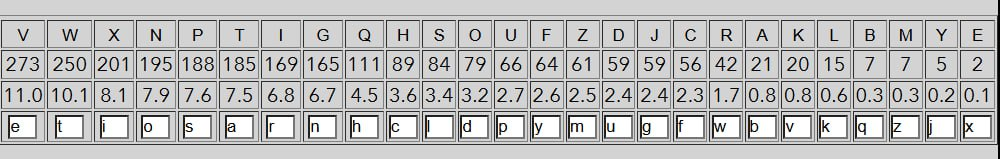
\includegraphics[width=0.8\textwidth]{img/final.jpg}
    \caption{The all decrypted letters}
    \label{fig:result1}
\end{figure}

% \section*{Results}
% \hspace{0.8cm}

% \textit{Task1}

% \begin{figure}[h!]
%     \centering
%     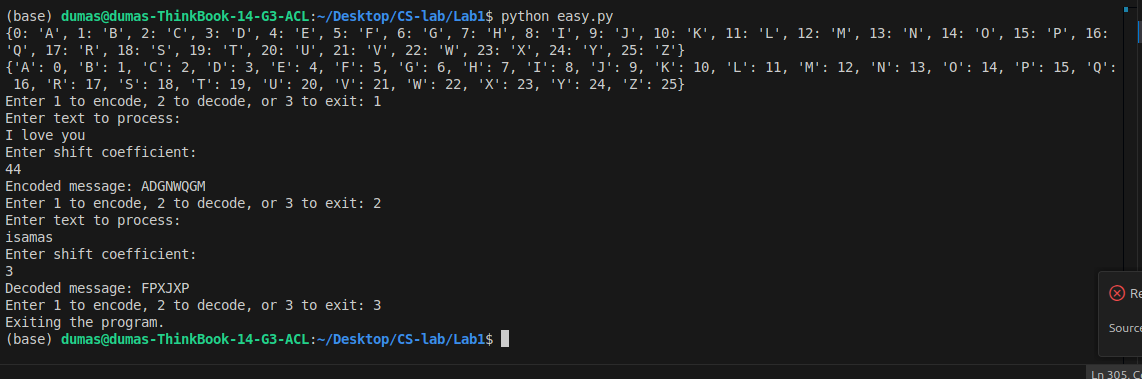
\includegraphics[width=0.8\textwidth]{img/Res1.png}
%     \caption{Result of the encoding and decoding program}
%     \label{fig:result1}
% \end{figure}

% \textit{Task2}

% \begin{figure}[h!]
%     \centering
%     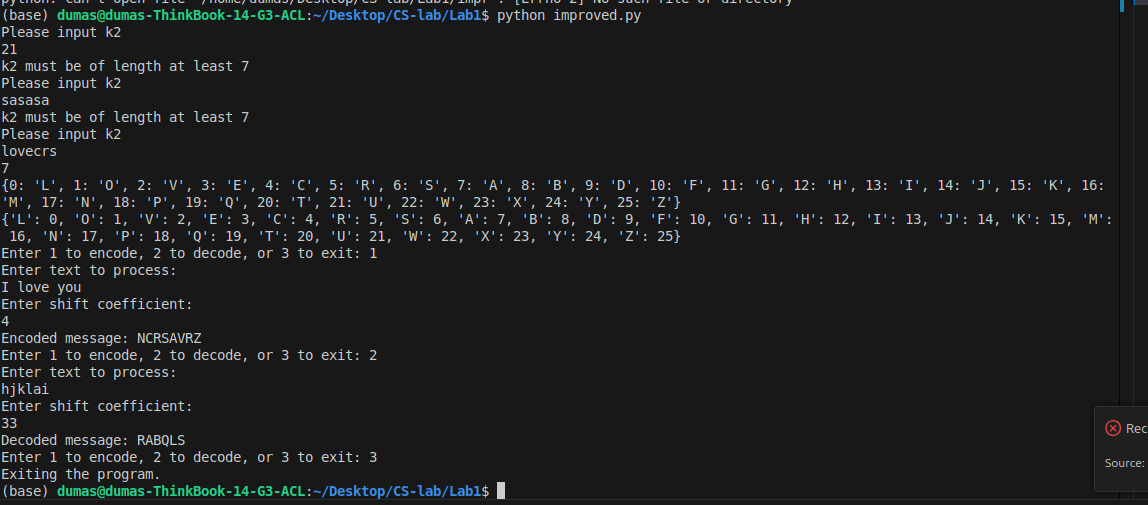
\includegraphics[width=0.8\textwidth]{img/Res2.png}
%     \caption{Result of the encoding and decoding program}
%     \label{fig:result1}
% \end{figure}





\section*{Conclusion}
\hspace{0.8cm}

In this laboratory work, we explored the principles of classical cryptography through the cryptanalysis of a monoalphabetic substitution cipher using frequency analysis. The primary objective was to decrypt an encrypted message by leveraging the statistical properties of the English language, specifically the characteristic frequency distribution of its letters.

The process began with calculating the frequency of each character in the ciphertext and comparing it to the standard frequency distribution of English letters. Initial substitutions were made by matching the most frequent letters in the ciphertext ('V' and 'W') with the most common English letters ('E' and 'T'). This foundational step allowed for the identification of common words and patterns, such as "the," which further revealed additional character mappings.

Through iterative analysis, digraph and trigraph frequencies, along with contextual clues, were used to progressively decrypt the message. Key steps included identifying single-letter words ("A" and "I"), common word structures, and frequently occurring pairs and triplets (e.g., "TH," "THE"). The manual nature of this process highlighted the importance of human intuition and linguistic knowledge in cryptanalysis, as purely algorithmic approaches may struggle with ambiguities and exceptions in natural language.

This exercise demonstrated the vulnerability of monoalphabetic ciphers to frequency analysis, especially with sufficiently long texts where statistical patterns emerge clearly. It also reinforced the importance of robust encryption methods that obscure these patterns to enhance security. Overall, the laboratory work provided valuable hands-on experience in classical cryptanalysis, illustrating the interplay between mathematics, linguistics, and logic in breaking substitution ciphers.
% \section*{Bibliography}
% \hspace{0.8cm}
% \begin{enumerate}
%   \item Resource 1
%   \item Resource 2
%   \item Resource 3 
% \end{enumerate}

\pagebreak
\end{document}